\begin{subsectionframemod}{Cross-Domain Few-Shot Object Detection}
        \metroset{block=fill}
    \vspace{-10mm}
    \begin{alertblock}{Détection d'objet few-shot cross-domain}
        Dans la détection d'objets à faible échantillon inter-domaines (CD-FSOD), deux ensembles de données distincts sont utilisés pendant l'entraînement de base et l'affinage.
        La CD-FSOD est plus difficile, car le modèle doit non seulement s'adapter à de nouvelles classes, mais aussi à de nouvelles images.
    \end{alertblock}
    \vspace{5mm}

    \pause

    \begin{center}
        \begin{tikzpicture}[
            squarednode/.style={rectangle, draw=black, thick, minimum size=5mm},
            node distance=20mm,
        ]
            % Nodes
            \node[squarednode, label=below:{\small Dataset de base}] (maintopic) {COCO Dataset};
            \node[squarednode, right= of maintopic] (rightsquare) {Modèle de détection};
%
%            % Lines
            \draw[->] (maintopic.east) -- node[above]{\small{Base Training}}(rightsquare.west);
        \end{tikzpicture}
    \end{center}

        \pause
    \begin{center}
        \begin{tikzpicture}[
            squarednode/.style={rectangle, draw=black, thick, minimum size=5mm},
            node distance=20mm,
        ]
            % Nodes
            \node[squarednode, label=below:{\small Dataset cible}] (maintopic) {DOTA Dataset};
            \node[squarednode, right= of maintopic] (rightsquare) {Modèl de détection};
%
%            % Lines
            \draw[->] (maintopic.east) -- node[above]{\small{Finetuning}}(rightsquare.west);
        \end{tikzpicture}
    \end{center}

%
%    \begin{tikzpicture}
%        \node[anchor=south west,inner sep=0, label=below:{\small Base Dataset}] at (0,0){
%            \fbox{\parbox[][10mm][c]{0.8\textwidth}{\centering\normalsize COCO Dataset}}
%        };
%    \end{tikzpicture}
%
%    \begin{columns}
%        \begin{column}{0.3\textwidth}
%            \centering
%
%            \begin{tikzpicture}
%                \node[anchor=south west,inner sep=0, label=below:{\small Target Dataset}] at (0,0){
%                    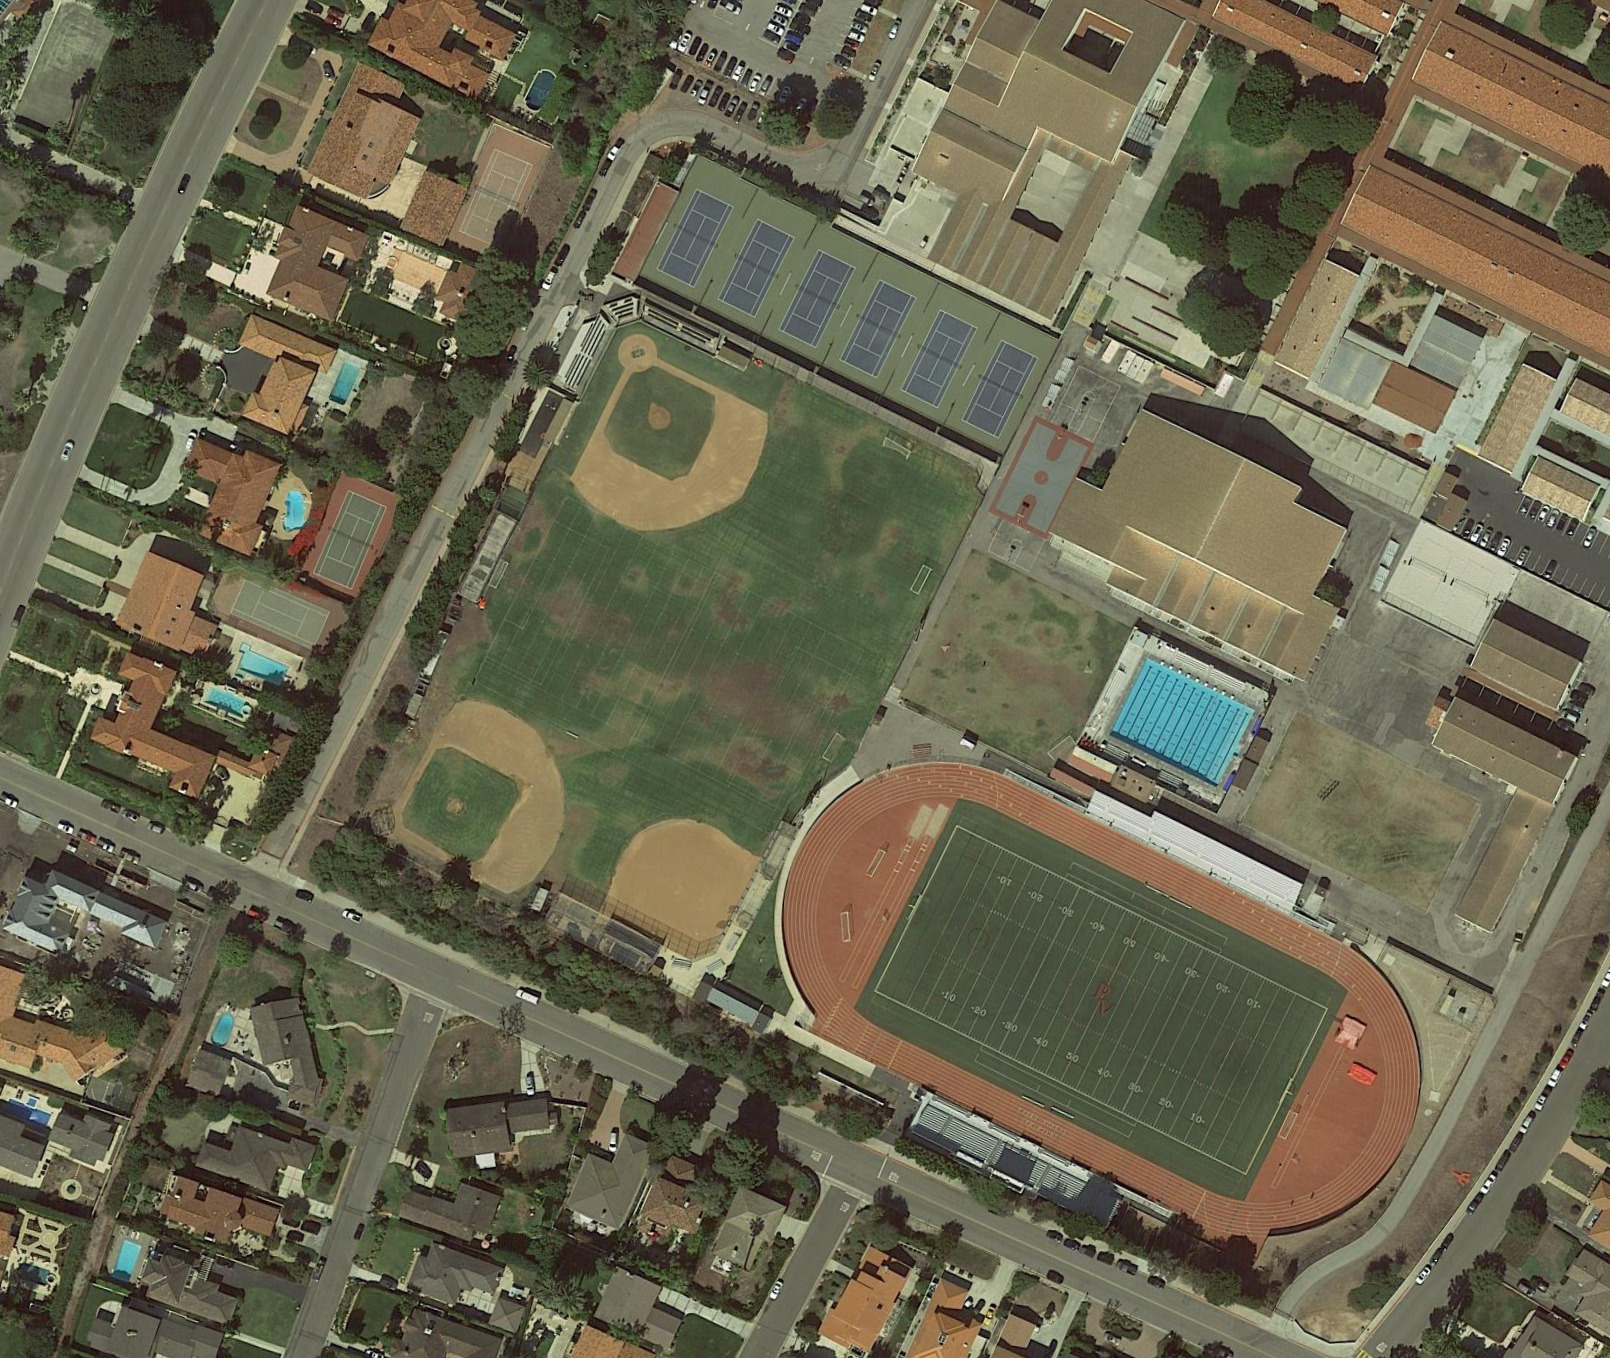
\includegraphics[width=30mm]{Figures/P0770}
%                };
%
%            \end{tikzpicture}
%
%        \end{column}
%        \pause
%
%        \begin{column}{0.3\textwidth}
%            \only<4->{
%                \begin{textblock*}{50mm}(57mm,53mm)
%                    \huge $\longrightarrow$\\
%                    \small {Base Training}
%                \end{textblock*}
%            }
%
%        \end{column}
%        \pause
%
%        \begin{column}{0.3\textwidth}
%            \only<4->{
%
%
%                \begin{tikzpicture}[remember picture,overlay]
%                    \node[anchor=south west,inner sep=0] at (0,0){%
%                        \fbox{\parbox[][10mm][c]{0.8\textwidth}{\centering\normalsize Detection model}}
%                    };
%                \end{tikzpicture}
%            }
%        \end{column}
%    \end{columns}

\end{subsectionframemod}